\scanpage{24}
\figure{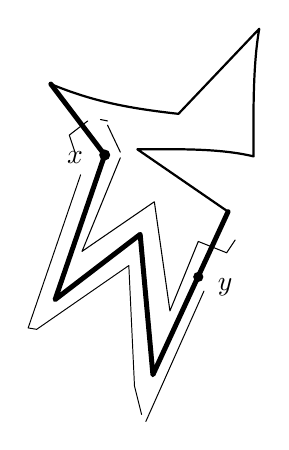
\begin{tikzpicture}[x=.018cm,y=-.018cm,line join=round,line cap=round]
\draw[line width=.8pt] (22,39)..controls (51,51) and (76,56)..(112,60)--(169,0)..controls (164,28) and (165,68)..(165,90)..controls (140,84) and (109,85)..(83,85)--(147,129);
\draw[line width=1.8pt] (22,39)--(60,89)--(25,191)--(85,145)--(94,244)--(147,129);
\draw[line width=.38pt] (48,65)--(35,75)--(39,87) (57,64)--(62,65) (62,68)--(71,87);
\draw[line width=.38pt] (71,91)--(44,157)--(95,122)--(106,199)--(126,150)--(146,158)--(152,149);
\draw[line width=.35pt] (43,103)--(6,211)--(12,212)--(77,167)--(81,252)--(86,272);
\draw[line width=.36pt] (89,277)--(130,185);
\fill (60,89) circle[radius=3.9];
\fill (126,175) circle[radius=3.6];
\node[inner sep=0pt] at (39,91) {$x$};
\node[inner sep=0pt] at (145,182) {$y$};
\end{tikzpicture}}

% The lower strip shows through horizontally reversed. The direction is restored
% here to read the three lines. Two lines carry a stroke through their text.
\margin{\tikz[x=.07cm,y=.07cm]{\draw (0,0)--(.1,-.6) (.15,-1.4)--(.1,-2.8);}}%
\uline{\unsure{Definition|Définition}} 3. Si $\Gamma$ est un polygone et $s,s'\in\mathbb{R}^{2}-\Gamma$ on dit que
\deleted{$s$ est visible de $s'$ ou bien que le couple \inserted{\unsure{de points} $s,s'$} est mutuellement visible si}

\margin{\tikz[x=.07cm,y=.07cm]{\draw (0,0)--(.12,-1) (.1,-1.45)--(-.14,-2.8);}}%
\margin{\tikz[x=.07cm,y=.07cm]{\draw (.15,0)..controls (.35,-.4) and (0,-.8)..(-.1,-1.2) (-.1,-1.5)..controls (0,-1.9) and (.1,-2.25)..(-.1,-2.7);}}%
\[
\deleted{\unsure{[s,s']|]s,s'[}\unsure{-|=}\{s,s'\}\unsure{\subset|\in}\mathbb{R}^{2}-\Gamma.}
\]
% archive sheet number: 23
